\section{Database}
\label{sec:database}
All tables will contain an \textsf{id} column, such that all rows in the same table are unique. This also makes it easy to fetch and perform actions for a specific row.

\textsf{users} table should at minimum contain the columns \textsf{username, password} and \textsf{email}.

\textsf{files} table should at minimum contain the columns \textsf{name, latitude, longitude, path, type} and \textsf{offset}.
Also, as it would be convenient to know who uploaded the file, a \textsf{user\_id} field should also be created.

There will be a table for all supported file types (currently \textsf{csv} and \textsf{wrk}). \textsf{csv} table should contain columns as stated in appendix \ref{ap:csv}, and \textsf{wrk} as defined by the VRIS\footnote{See \cite{VRIS} for definition} file format. Besides these columns, all file type tables should contain a \textsf{file\_id} field so all data is related to the source file (in the database).

As the database should be able to handle a large amount of data, it is crucial that all columns are of correct and optimal data types, e.g. \textsf{id} columns are either \textit{int} or \textsf{bigint} and are \textsf{unsigned}. By comparison, \textsf{unsigned int} can take the maximum value $2^{32}-1 (\approx 4.29 \cdot 10^{9})$ while it for \textsf{unsigned bigint} is $ 2^{64}-1 (\approx 18.45 \cdot 10^{18})$.

Figure \ref{fig:dbdiagram} is a diagram of the database has been implemented based on the analysis and design.

\begin{figure}[htbp]
   \centering
   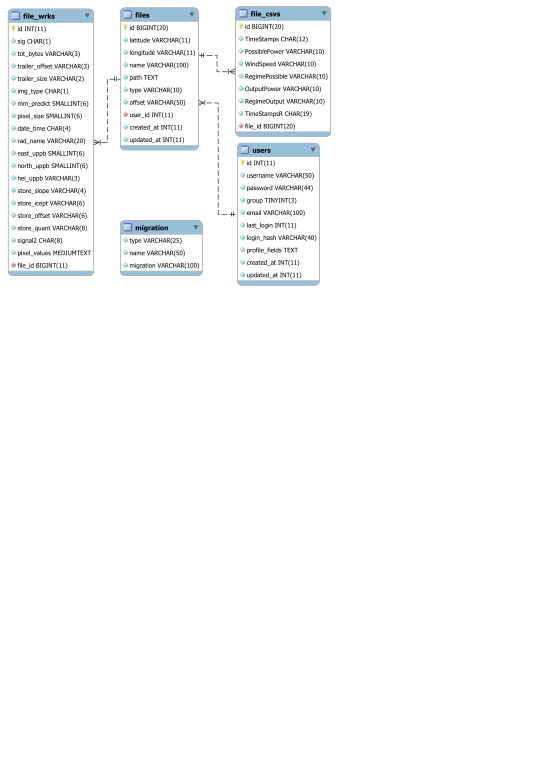
\includegraphics[width=1\linewidth]{figure/db}
   \caption{Database Diagram}
   \label{fig:dbdiagram}
\end{figure}

FuelPHP contains a \textsf{migration} tool that lets one create revisions for the database, hence easy deployment of changes. This tool has been used to create all tables, and therefore the \textsf{migration} table is used to keep track of revisions.

All tables use \textsf{InnoDB}, because this engine make it possible to create sql relations. This means that if a table has a foreign key (i.e. a key that identifies a row in another table), one can create actions for what should happen to the rows in the current table, if the related row in the other table is \textsf{updated} or \textsf{deleted}.

These relations can be seen in the diagram. The relations and actions is stated by sql as in listing \ref{lst:sql}
\begin{lstlisting}[language=sql,caption={SQL realations and actions},label={lst:sql}]
ALTER TABLE `files`
  ADD CONSTRAINT `files_ibfk_1` FOREIGN KEY (`user_id`) REFERENCES `users` (`id`) ON DELETE NO ACTION ON UPDATE NO ACTION;

ALTER TABLE `file_csvs`
  ADD CONSTRAINT `file_csvs_ibfk_1` FOREIGN KEY (`file_id`) REFERENCES `files` (`id`) ON DELETE CASCADE ON UPDATE NO ACTION;

ALTER TABLE `file_wrks`
  ADD CONSTRAINT `file_wrks_ibfk_1` FOREIGN KEY (`file_id`) REFERENCES `files` (`id`) ON DELETE CASCADE ON UPDATE NO ACTION;
\end{lstlisting}

\subsection{Optimization}
\label{sec:database_optimization}
In FuelPHP it is possible to create model relations that are similar to sql relations with actions, but easier to manage and at the same time less efficient (though generally adequate). This method was used initially, but performance was found to be too bad, e.g. it would take too much time to cascade delete all the csv rows related to the file selected for deletion, eventually leading to a time out by the server. The time out limit can be changed by the server manager, but it was easier and - as stated before - more efficient to make relation actions in sql. Relations are still present at model level, but actions have been turned off.

When first creating the database, the data types for the fields were not optimized, and as previously stated this is important for performance, and improper data types or constraints can even break the data that should be saved. When optimising the data types, we were also able to gain space and e.g. halve the size of the \textsf{file\_csvs} from maximum 372 bytes per row to maximum 107 bytes.

As seen on figure \ref{fig:dbdiagram}, \textsf{id} for  \textsf{files, file\_csvs} and  \textsf{file\_wrks} are of type \textsf{bigint} ( \textsf{unsigned}). This make it possible for these tables to store a huge amount of data, and even though \textsf{unsigned int} can save a large amount too, we would rather make the application future proof than let it break if the limit was reached.

Equations \ref{eq:db_1} through \ref{eq:db_4} illustrate the problem and reason for the decision made.

\emph{Number of csv files stored, if the data is represented by a 10 minute interval in a span of 1.5 years (as current test data):}

\textsf{unsigned int}: 
\begin{equation}
\label{eq:db_1}
\left\lfloor \frac{2^{32}-1}{72,858} \right\rfloor = 58,949
\end{equation}

\textsf{unsigned bigint}:
\begin{equation}
\label{eq:db_2}
\left\lfloor \frac{2^{64}-1}{72,858} \right\rfloor = 253,187,626,255,312
\end{equation}

\emph{Number of csv files stored, if the data is represented by a 1 minute interval in a span of 1.5 years:}

\textsf{unsigned int}:
\begin{equation}
\label{eq:db_3}
\left\lfloor \frac{2^{32}-1}{72,858 \cdot 10} \right\rfloor = 5,894
\end{equation}

\textsf{unsigned bigint}:
\begin{equation}
\label{eq:db_4}
\left\lfloor \frac{2^{64}-1}{72,858 \cdot 10} \right\rfloor = 25,318,762,625,531
\end{equation}

As the storage size of \textsf{bigint} is only twice as big as \textsf{int}, the maximum increase in storage per row is not remarkable, where as the increase in number of possible files storeable is increased by a huge margin as seen on equation \ref{eq:db_3} and \ref{eq:db_4}.